\chapter{Electrodynamics of spinless particles}
\begin{enumerate}[1)]
    \item Introduction of charged particle in potential
    \item Potential provided by the other scattering matter
\end{enumerate}

\section{Covariant electrodynamics}
From electrodynamics recall Maxwell's equation:
\begin{align*}
    \vec \grad \vec E & = \rho   & \vec \grad \times \vec E & = - \pa_t \vec B \\
    \vec \grad \vec B & = 0      & \vec \grad \times \vec B & = \vec j + \pa_t \vec E
\end{align*}
Express the fields $\vec E$, $\vec B$ by potentials $\phi$, $\vec A$:
\begin{align}
    \vec B = \vec \grad \times \vec A, \qquad \vec E = - \vec \grad \phi - \pa_t \vec A
\end{align}
Gauge freedom: Choose Coulomb gauge? $\vec \grad \vec A = 0$\\
Here: We will use the Lorentz gauge $\boxed{\vec \grad \vec A + \pa_t \phi = 0}$
\begin{align}
    & \Ra \quad \Lap \vec A - \pa_t^2 \vec A = - \vec j, \qquad \Lap \phi - \pa_t^2 \phi = - \rho
\end{align}
With $A^\mu \ra \qty(-\phi, \vec A)$ and $j^\mu \ra \qty(\rho, \vec j)$, we get Maxwell's equations in covariant form
\begin{align}
    \boxed{ \pa_\mu \pa^\mu A^\nu = j^\nu }\,.
\end{align}
Not that the Lorentz gauge can also be written as $\boxed{\pa_\mu A^\mu = 0 = \pa^\mu A_\mu}$.

\section{The spinless electron in the electromagnetic field}
In classical electrodynamics the canonical momentum is
\begin{align}
    \begin{rcases} E \ra E - Q \phi \\ \vec p \ra \vec p - Q \vec A \end{rcases} \qquad p^\mu \ra p^\mu - Q A^\mu\,.
\end{align}
We will substitute by operators:
\begin{align}
    \begin{rcases} E - Q \phi \ra \ti \pa_t - Q \phi \\ \vec p - Q \vec A \ra - \ti \vec \grad - Q \vec A \end{rcases} \qquad \ti \pa^\mu - Q A^\mu
\end{align}
In total, for electrons of charge $Q= -\mr e$:
\begin{align}
    \boxed{p^\mu \ra \ti \pa^\mu + \mr e A^\mu}
\end{align}
By insertion into Klein-Gordon equation (see \cref{eq:KGe}):
\begin{align}\begin{split}
    & \qty(\ti \pa_\mu + \mr e A_\mu) \qty(\ti \pa^\mu + \mr e A^\mu) \phi\qty(\fvec x) - m^2 \phi \qty(\fvec x) = 0 \\
    & H_0 \ra H_0 + V \\
    & \Ra \quad \bigg( \pa_\mu\pa^\mu \underbrace{- \ti \mr e \qty(A_\mu \pa^\mu + \pa_\mu A^\mu ) - \mr e^2 A^2 + m^2}_{V_\mr{EM}} \bigg) \phi \qty(\fvec x) = 0
\end{split}\end{align}
Perturbation of free particle Hamiltonian $H_0$ due to the coupling of electron to $A^\mu$. We are only interested in the leading order contribution $\ra$ neglect the term $\propto \mr e^2$
\begin{align}
    \boxed{ V_\mr{EM} \qty(\fvec x) = - \ti \mr e \qty(\pa_\mu A^\mu + A_\mu \pa^\mu) }
\end{align}
with this the charge current density is
\begin{align}
    j^\mu = - \ti \mr e \qty( \phi_\mr{f}^* \pa^\mu \phi_\mr{i} - \qty( \pa_\mu \phi_\mr{f}^*) \phi_\mr{i} )
\end{align}
\begin{center}
    \begin{tikzpicture}
        \begin{feynman}
            \vertex (b1);
            \vertex [above left = 1.5cm of b1] (a1) {$\phi_\mr{i}$};
            \vertex [above right = 1.5cm of b1] (a2) {$\phi_\mr{f}$};
            \vertex [below = 1cm of b1] (c1) {$V\qty(\fvec x)$};
            \vertex [right = 1cm of a1] (j1);
            \vertex [left = 1cm of a2] (j2);
            \diagram*{
            (a1) -- [fermion] (b1) -- [fermion] (a2);
            (b1) -- [photon] (c1);
            (j1) -- [draw = none, momentum' = $\ $, edge label = $j^\mu$, half right] (j2);
            };
        \end{feynman}
    \end{tikzpicture}
\end{center}
\begin{align}\begin{split}
    T_\mr{fi} & = - \ti \int \phi_\mr{f}^* \qty(\fvec x) V_\mr{EM} \qty(\fvec x) \phi_\mr{i}\qty(\fvec x) \dd[4]{x} \\
    & = - \ti \int \qty(-\ti \mr e) \phi_\mr{f}^* \qty(\pa_\mu A^\mu + A_\mu \pa^\mu) \phi_\mr{i} \dd[4]{x}
\end{split}\end{align}
with integration by parts
\begin{align}
    \int\limits_{-\infty}^{\infty} \phi_\mr{f}^* \pa_\mu A^\mu \phi_\mr{i} \dd[4]{x} = \underbrace{\qty[\phi_\mr{f}^* \sum_\mu A^\mu \phi_\mr{i}]_{-\infty}^{\infty}}_{=0} - \int\limits_{-\infty}^{\infty} \qty(\pa_\mu \phi_\mr{f}^*) A^\mu \phi_\mr{i} \dd[4]{x}
\end{align}
hence
\begin{align}\begin{split}\label{eq:transition_amplitude_tree}
    T_\mr{fi} & = -\ti \int \qty(-\ti \mr e) \qty[ - \qty(\pa_\mu \phi_\mr{f}^*) A^\mu \phi_\mr{i} + \phi_\mr{f}^* A^\mu \pa_\mu \phi_\mr{i} ] \dd[4]{x} \\
    & = - \ti \int \underbrace{\overbrace{\qty(-\ti\mr e)}^{\substack{\text{coupling}\\\text{constant}}} \qty[ \phi_\mr{f}^* \pa_\mu \phi_\mr{i} - \qty(\pa_\mu \phi_\mr{f}^*) \phi_\mr{i} ]}_{\substack{\text{four vector current of} \\ \text{an electron (see \cref{eq:four_density_KGe}}}} \underbrace{\ A^\mu\ }_{\mathrlap{\substack{\text{interaction} \\ \text{four potential}}}} \dd[4]{x}\\
    \Aboxed{ T_\mr{fi} & = -\ti \int j_\mu^G A^\mu \dd[4]{x}}
\end{split}\end{align}
The boxed equation gives us the coupling between electron charge current and electromagnetic potential with coupling strenth $\mr e$.\\
$\ra$ The Feynman diagram can be extended with new information:
\begin{center}
    \begin{tikzpicture}
        \begin{feynman}
            \vertex (b1);
            \vertex [above left = 2cm of b1] (a1) {$\mr e^-$};
            \vertex [above right = 2cm of b1] (a2) {$\mr e^-$};
            \vertex [below = 1cm of b1] (c1) {$A^\mu$};
            \vertex [right = 1cm of a1] (j1);
            \vertex [left = 1cm of a2] (j2);
            \diagram*{
            (a1) [particle = $\mr e^-$] -- [fermion] (b1) -- [fermion] (a2);
            (b1) -- [photon] (c1);
            (j1) -- [draw = none, momentum' = $\ $, edge label = $j_\mu^G \qty(\mr e^-)$, half right] (j2);
            };
        \end{feynman}
    \end{tikzpicture}
\end{center}
Free-particle approximation:\todo[color = none]{Similar calculation can be done for $u,c,t \ra \frac 23 \mr e$ and $d,s,b \ra - \frac 13 \mr e$}
\begin{align}\begin{split}
    & \phi_\mr{i}\qty(\fvec x) = N_\mr{i} \exp(- \ti \fvec p_\mr{i} \fvec x), \qquad \phi_\mr{f} \qty(\fvec x) = N_\mr{f} \exp(- \ti \fvec p_\mr{f} \fvec x) \\
    & \Ra \quad \boxed{ j_\mu^\mr{fi} \qty(\fvec x) = - \mr e N_\mr{i} N_\mr{f} \qty(\fvec p_\mr{i} + \fvec p_\mr{f})_\mu \exp(-\ti \qty(\fvec p_\mr{i} - \fvec p_\mr{f}) \fvec x) }
\end{split}\end{align}
This denotes the charge density current of scattering an electron in free-particle  approximation.

\pagebreak
\section{Spinless electron-muon scattering}
The electromagnetic potential $A^\mu$ now is provided by a $\mu$-current. Thus the Feynman diagram is

\begin{center}
    \begin{tikzpicture}
        \begin{feynman}
            \vertex (b1);
            \vertex [above left = 2cm of b1] (a1) {$\mr e^-$};
            \vertex [above right = 2cm of b1] (a2) {$\mr e^-$};
            \vertex [below = 1cm of b1] (c1) {$A^\mu$};
            \vertex [right = 1cm of a1] (j1);
            \vertex [left = 1cm of a2] (j2);
            \diagram*{
            (a1) [particle = $\mr e^-$] -- [fermion] (b1) -- [fermion] (a2);
            (b1) -- [photon] (c1);
            (j1) -- [draw = none, momentum' = $\ $, edge label = $j_\mu^G \qty(\mr e^-)$, half right] (j2);
            };
            \vertex [right = 6cm of a1] (z1) {$\mr e^-$};
            \vertex [below right = 2.5cm of z1] (y1);
            \vertex [above right = 2cm of y1] (z2) {$\mr e^-$};
            \vertex [below = 1.5cm of y1] (x1);
            \vertex [below left = 2cm of x1] (w1) {$\upmu^-$};
            \vertex [below right = 2cm of x1] (w2) {$\upmu^-$};
            \vertex [right = 1cm of w1] (k1);
            \vertex [left = 1cm of w2] (k2);
            \vertex [right = 1cm of z1] (l1);
            \vertex [left = 1cm of z2] (l2);
            \diagram*{
            (z1) -- [fermion, momentum' = $\fvec p_A$] (y1) -- [fermion, momentum' = $\fvec p_C$] (z2);
            (y1) -- [photon, edge label' = $\upgamma$] (x1);
            (w1) -- [fermion, momentum = $\fvec p_B$] (x1) -- [fermion, momentum = $\fvec p_D$] (w2);
            (l1) -- [draw = none, half right, momentum' = $\ $, edge label = $j_\nu^{(1)}$] (l2);
            (k2) -- [draw = none, half right, rmomentum' = $\ $, edge label = $j_\nu^{(2)}$] (k1);
            };
        \end{feynman}
    \end{tikzpicture}
\end{center}

Connection between potential $A^\mu$ and $\mu$-current $j_\mu^{(2)}$ vie Maxwell relation
\begin{align}
    \pa_\mu \pa^\mu A^\nu = j_{(2)}^\nu 
\end{align}
where
\todo[color=none]{Note that this is the charge density current of a muon in the free-particle approximation.}
\begin{align}
    j_{(2)}^\nu = - \mr e N_B N_D \qty( \fvec p_B + \fvec p_D)^\nu \exp( - \ti \qty(\fvec p_B - \fvec p_D) \fvec x)\\
    \ra \quad \pa_\mu \pa^\mu A^\nu = - \mr e N_B N_D \qty(\fvec p_B + \fvec p_D)^\nu \exp(\ti \fvec q \fvec x)
\end{align}
since $q^\mu = \qty(\fvec p_A - \fvec p_C)^\mu = \qty(\fvec p_B - \fvec p_D)^\mu$.

The solution for the four potential is
\begin{align}
    \boxed{A^\mu \qty(\fvec x) = - \frac{1}{\fvec q^2} j_{(2)}^\mu \qty(\fvec x)}\,,
\end{align}
which is the electromagnetic potential due to fly-by muon.

Transition amplitude on tree level (see \cref{eq:transition_amplitude_tree}):
\begin{align}
    T_\mr{fi} = -\ti \int j_\mu^{(1)} \qty(\fvec x) A^\mu \qty(\fvec x) \dd[4]{x} = -\ti \int j_\mu^{(1)} \qty(\fvec x) \qty(-\frac{1}{\fvec q^2}) j_{(2)}^\mu \qty(\fvec x) \dd[4]{x}
\end{align}
Integration similiar to \cref{sec:Interaction_particle_potential}:
\begin{align}
    T_\mr{fi} = - \ti \underbrace{N_A N_B N_C N_D}_{\substack{\text{wave functions} \\ \text{normalisation}}} \qty(2\pi)^4 \underbrace{\delta^4 \qty(\fvec p_D + \fvec p_C - \fvec p_B - \fvec p_A)}_{\substack{\text{component-wise}\\ \text{energy-momentum conservation}}} m
\end{align}
With the \tb{invariant amplitude $m$} being
\begin{align}
    -\ti m = \underbrace{\ti \mr{e} \qty(\fvec p_A + \fvec p_C)^\mu}_{\substack{\text{electron current} \\ \text{(coupling const. $\mr e$)}}} \underbrace{\qty(- \frac{\ti}{\fvec q^2} \tensor{g}{_\mu_\nu})}_{\substack{\text{photon} \\ \text{propagator}}} \underbrace{\ti \mr e \qty(\fvec p_B + \fvec p_D)^\nu}_{\substack{\text{muon current} \\ \text{(coupling const. $\mr e$)}}} \,.
\end{align}
$m$ describes the physics of the process:
\begin{center}
    \begin{tikzpicture}
        \begin{feynman}
            \vertex (y1);
            \vertex [above left = 2cm of y1] (z1) {$\mr e^-$};
            \vertex [above right = 2cm of y1] (z2) {$\mr e^-$};
            \vertex [below = 1.5cm of y1] (x1);
            \vertex [below left = 2cm of x1] (w1) {$\upmu^-$};
            \vertex [below right = 2cm of x1] (w2) {$\upmu^-$};
            \vertex [right = 1cm of w1] (k1);
            \vertex [left = 1cm of w2] (k2);
            \vertex [right = 1cm of z1] (l1);
            \vertex [left = 1cm of z2] (l2);
            \diagram*{
            (z1) -- [fermion, momentum' = $\fvec p_A$] (y1) -- [fermion, momentum' = $\fvec p_C$] (z2);
            (y1) -- [photon, edge label' = $\upgamma$] (x1);
            (w1) -- [fermion, momentum = $\fvec p_B$] (x1) -- [fermion, momentum = $\fvec p_D$] (w2);
            (l1) -- [draw = none, half right, momentum' = $\ $, edge label = \scriptsize{$\mqty{j^\nu_{(1)} = \\ \ti \mr e \qty(\fvec p_A + \fvec p_C)^\nu}$}] (l2);
            (k2) -- [draw = none, half right, rmomentum' = $\ $, edge label = \scriptsize{$\mqty{j^\nu_{(2)} = \\ \ti \mr e \qty(\fvec p_B + \fvec p_D)^\nu}$}] (k1);
            };
        \end{feynman}
    \end{tikzpicture}
\end{center}
FOr some processes many realisations are possible, e.g.
\begin{align}
    \feynmandiagram[vertical = b to d, baseline = -1.4cm, small]{
        a [particle = $\mr e^-$] -- [fermion] b -- [fermion] c [particle = $\mr e^-$],
        b -- [photon] d,
        e [particle = $\mr e^+$] -- [anti fermion] d -- [anti fermion] f [particle = $\mr e^+$],
    };
    +
    \feynmandiagram[horizontal = b to d, baseline =(b.base),small]{
        a [particle = $\mr e^+$] -- [anti fermion] b -- [anti fermion] c [particle = $\mr e^-$],
        b -- [photon] d,
        e [particle = $\mr e^+$] -- [fermion] d -- [fermion] f [particle = $\mr e^-$],
    };
    \quad \longrightarrow \quad \qty|T_\mr{fi}^{(1)} + T_\mr{fi}^{(2)}|^2
\end{align}

\section{Towards the \texorpdfstring{$\mr e^- \upmu^- \ra \mr e^- \upmu^-$}{} cross section}
Wave function: $hi \qty(\fvec x) = N \exp(-\ti \fvec p \fvec x)$; Probability density: $\rho = 2E \qty|N|^2$

The probability to find a particle in arbitrary (large) volume $V$: $\int_V \rho \dd[e]{x} \overset{!}{=} 1$
\begin{align}
    \ra \quad N = \frac{1}{\sqrt{2EV}}\,,
\end{align}
which is the covariant normalisation. Accordingly, the transition rate is:
\begin{align}
    W_\mr{fi} = \Gamma_\mr{fi} = \frac{\qty| T_\mr{fi}|^2}{TV} = \qty(16 V^4 E_A E_B E_C E_D) \qty(2\pi)^4 \delta^4 \qty(\fvec p_D + \fvec p_B - \fvec p_A - \fvec p_C) \qty|m|^2
\end{align}
In the next step, we want to calculate the cross section. This resembles the effective area that a particle sees from a target when undergoing scattering.
\begin{align}
    \qty[\sigma] = \si{\square\meter}, \qquad \SI{1}{\barn} = \SI{e-28}{\square\meter}
\end{align}
So what is the cross section for a process $AB \ra CD$?

In the laboratory system:
\begin{center}
    \begin{tikzpicture}
        \draw[thick, -latex] (0,0) node [left] {$N_A$} -- node [above] {$\vec v_A$} (3,0);
        \draw (3.1,-1.5) rectangle (3.3,1.5);
        \draw[thick, -latex] (3.4,0.15) -- (6.4,1.55) node [right] {$\dd{N_C} = \dd{N_A}$};
        \draw[thick, dashed,-latex] (3.4,0) -- (6.4,0) node [right] {$N_A - \dd{N_A}$};
        \node [below] at (3.2,-1.5) {$n_B$};
        \node [above] at (3.2,1.5) {$\rightarrow \dd{x} \leftarrow$}; 
    \end{tikzpicture}
\end{center}
absorption:
\begin{align}
    \dd{N_A} = - N_A \frac{\dd{x}}{\lambda} = -N_A \dd{x} n_B \sigma
\end{align}
\begin{compactitem}
    \item[with] $\lambda$: scattering length
    \item[] $\sigma$: cross section
    \item[] $n_B$: target density
\end{compactitem}
\begin{align}
    \ra \quad N_A \qty(\Delta x) = N_A \qty(0) \mr e^{-n_B \sigma \Delta x} \approx N_A\qty(0) \qty(1-n_B \sigma \Delta x)
\end{align}
From the setup it is clear that the number of absorbed particles is the same as the number of scattered particles. Thus:
\begin{align}
    N_C \qty(\Delta x) = N_A\qty(0) n_B \Delta x \cdot \sigma = L \cdot \sigma 
\end{align}
Here we define the \tb{integrated luminsity} $L$ ($\qty[L] = \si{\per\square\meter}$). It covers beam and target-related properties.

\paragraph{Connection to the transition rate $W_\mr{fi}$?}
Consider the interaction of particles $A$ and $B$ in volume $V$:
\begin{center}
    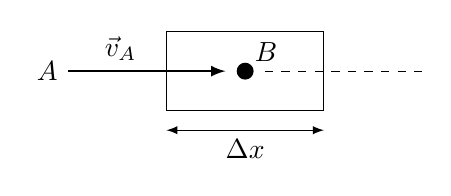
\begin{tikzpicture}
        \draw[thick, -latex] (0,0) node [left] {$A$} -- node [above left] {$\vec v_A$} (2,0);
        \draw[fill=black] (2.25,0) circle (0.1) node [above right] {$B$};
        \draw (1.25,-0.5) rectangle (3.25,0.5);
        \draw[latex-latex] (1.25,-0.75) -- node [below] {$\Delta x$} (3.25,-0.75);
        \draw[dashed] (2.5,0) -- (4.5,0);
    \end{tikzpicture}
\end{center}
The interaction time (particle $A$ is in $V$):
\begin{align}
    \Delta T & = \frac{\Delta x}{\qty|\vec v_A|} \nonumber \\
    \sigma & = \frac{N_C}{L} = \frac{N_C}{\Delta T\, V}\frac{\Delta T \, V}{N_A \Delta x \, n_B} = W_\mr{fi} \frac{1}{n_A} \frac{1}{\qty|\vec v_A|} \frac{1}{n_B} \qty(\# \text{final states}) \nonumber \\
    & \ra \quad \boxed{\sigma = \frac{W_\mr{fi}}{n_A \qty|\vec v_A| n_B} \qty(\# \text{final states}) }
\end{align}
\begin{compactitem}
    \item[with] $n_A \qty|\vec v_A|$: flux density of particles A (dimension: \si{\per \square \meter \per \second})
    \item[] $n_A = n_B = \nicefrac 1V$: one particle each in the volume
\end{compactitem}

\paragraph{What is the number of final states?}
Assuming fermions, each final state particle occupies phase volume $\mr h^3 = \qty(2\pi \hbar)^3$ in 6-dimensional phase space
\begin{align}
    \# \text{states} = \frac{V \dd[3]{p}}{\qty(2\pi \hbar)^3} \cdot \underbrace{\frac{1}{\# \text{particles in } V}}_{\substack{\equiv 1 \text{ (wave} \\ \text{function normalisation)}}}\,.
\end{align}
The cross section $\dd{\sigma}$ for scattering final states into momentum elements $\dd[3]{p_C} \dd[3]{p_D}$
\begin{align}
    \dd{\sigma} & = \frac{W_\mr{fi} V^2}{\qty|\vec v_A|} \cdot \frac{V \dd[3]{p_C}}{\qty(2\pi)^3}\frac{V \dd[3]{p_D}}{\qty(2\pi)^3} \nonumber \\
    & = \underbrace{\frac{1}{\qty|\vec v_A| 2 E_A 2 E_B}}_{\text{flux factor } \mc F} \qty|m|^2 \underbrace{\qty(2\pi)^4 \delta^4 \qty(\fvec p_C + \fvec p_D - \fvec p_A - \fvec p_B) \frac{\dd[3]{p_C} \dd[3]{p_D}}{\qty(2\pi)^6} \frac{1}{E_C E_D}}_\text{Lorentz-invariant phase space factor}
\end{align}
The flux factor transfers all properties of incoming particles. In short the above expression is
\begin{align}
    \dd{\sigma} = \frac{\qty|m|^2}{\mc F} \dd{Q}\,.
\end{align}
For general colinear collisions:
\begin{align}
    \mc F = 4 \sqrt{\qty(\fvec p_A \fvec p_B)^2 - m_A^2 m_B^2}
\end{align}
This factor additionally is Lorentz-invariant. In the centre-of-mass system (CMS):
\begin{align}
    \boxed{\mc F = 4 \qty| \vec p_A| \sqrt s = 4 \qty|\vec p_i| \sqrt s}\\
    (\text{for } \vec p_A = - \vec p_B, \ \qty|\vec p_A| = \qty|\vec p_B| = \qty|\vec p_i|)\nonumber 
\end{align}
